\documentclass[final]{fhnwreport}       %[mode] = draft or final
                                        %{class} = fhnwreport, article, 
                                        %          report, book, beamer, standalone
%%---Main Packages-----------------------------------------------------------------------
\usepackage[english, ngerman]{babel}	%Mul­tilin­gual sup­port for LaTeX
\usepackage[T1]{fontenc}				%Stan­dard pack­age for se­lect­ing font en­cod­ings
\usepackage[utf8]{inputenc}				%Ac­cept dif­fer­ent in­put en­cod­ings
\usepackage{lmodern}                    %The newer Font-Set
\usepackage{textcomp}					%LaTeX sup­port for the Text Com­pan­ion fonts
\usepackage{graphicx} 					%En­hanced sup­port for graph­ics
\usepackage{float}						%Im­proved in­ter­face for float­ing ob­jects
\usepackage{ifdraft}                    %Let you check if the doc is in draft mode

%%---Useful Packages---------------------------------------------------------------------
\usepackage[pdftex,dvipsnames,table]{xcolor}  %Driver-in­de­pen­dent color ex­ten­sions for LaTeX
\usepackage{csquotes}                   %Simpler quoting with \enquote{}
\usepackage{siunitx} 					%A com­pre­hen­sive (SI) units pack­age
\usepackage{listings}					%Type­set source code list­ings us­ing LaTeX
\usepackage[bottom]{footmisc}			%A range of foot­note op­tions
\usepackage{footnote}					%Im­prove on LaTeX's foot­note han­dling
\usepackage{verbatim}					%Reim­ple­men­ta­tion of and ex­ten­sions to LaTeX ver­ba­tim
\usepackage[textsize=footnotesize]{todonotes} %Mark­ing things to do in a LaTeX doc­u­ment
\usepackage{booktabs}
\usepackage{lscape}
\usepackage{blindtext}
\usepackage{wrapfig}

%%---Tikz Packages-----------------------------------------------------------------------
\usepackage{standalone}
\usepackage{tikz}
\usepackage{circuitikz}
\usetikzlibrary{arrows}
\usetikzlibrary{calc}
\usetikzlibrary{intersections}

%%---Math Packages-----------------------------------------------------------------------
\usepackage{amsmath}					%AMS math­e­mat­i­cal fa­cil­i­ties for LaTeX
%\usepackage{amssymb}					%Type­set­ting symbols (AMS style)
%\usepackage{array}						%Ex­tend­ing the ar­ray and tab­u­lar en­vi­ron­ments
%\usepackage{amsthm}					%Type­set­ting the­o­rems (AMS style)

%%---Table Packages----------------------------------------------------------------------
\usepackage{tabularx}					%Tab­u­lars with ad­justable-width columns
%\usepackage{longtable}
\usepackage{multirow}					%Create tab­u­lar cells span­ning mul­ti­ple rows
\usepackage{multicol}					%In­ter­mix sin­gle and mul­ti­ple columns

%%---PDF / Figure Packages---------------------------------------------------------------
\usepackage{pdfpages}					%In­clude PDF doc­u­ments in LaTeX
\usepackage{pdflscape}					%Make land­scape pages dis­play as land­scape
\usepackage{subfig}					    %Fig­ures di­vided into sub­fig­ures

%%---Other Packages----------------------------------------------------------------------
%\usepackage{xargs}                     %De­fine com­mands with many op­tional ar­gu­ments

%%---Bibliography------------------------------------------------------------------------
\bibliographystyle{unsrt}

%%---Main Settings-----------------------------------------------------------------------
\graphicspath{{./graphics/}}			%Defines the graphicspath
%\geometry{twoside=false}				    %twoside=false disables the "bookstyle"
\setlength{\marginparwidth}{2cm}
\overfullrule=5em						%Creates a black rule if text goes over the margins => debugging


%%---User Definitions--------------------------------------------------------------------
%%Tabel-Definitions: (requires \usepackage{tabularx})
\newcolumntype{L}[1]{>{\raggedright\arraybackslash}p{#1}}    %column-width and alignment
\newcolumntype{C}[1]{>{\centering\arraybackslash}p{#1}}
\newcolumntype{R}[1]{>{\raggedleft\arraybackslash}p{#1}}

%%---Optional Package Settings-----------------------------------------------------------
%Listings-Settings: (requires \usepackage{listings}) => Example with Matlab Code
\lstset{language=Matlab,%
    basicstyle=\footnotesize\ttfamily,
    breaklines=false,%
    morekeywords={switch, case, otherwise},
    keywordstyle=\color{Blue},%
    tabsize=2,
    %morekeywords=[2]{1}, keywordstyle=[2]{\color{black}},
    identifierstyle=\color{Black},%
    stringstyle=\color{Purple},
    commentstyle=\color{Green},%
    showstringspaces=false,%without this there will be a symbol in the places where there is a space
    numbers=left,%
    numberstyle={\tiny \color{black}},% size of the numbers
    numbersep=9pt, % this defines how far the numbers are from the text
    %emph=[1]{word1, word2,...},emphstyle=[1]\color{red}
}										                %loads all packages, definitions and settings												
\title{\Huge{\textbf{Pflichtenheft}}\\}          %Project Title
\author{\huge{Wetterstation mit Solar Energie}}          %Document Type => Technical Report, ...
\date{Windisch, \today}             %Place and Date


\begin{document}


%%---TITLEPAGE---------------------------------------------------------------------------
\selectlanguage{ngerman}                %ngerman or english
\maketitle
%\vspace*{-1cm}
\vspace*{-0.5cm}						    %compensates the space after the date line.
\vfill
\begin{figure}[H]
\centering
%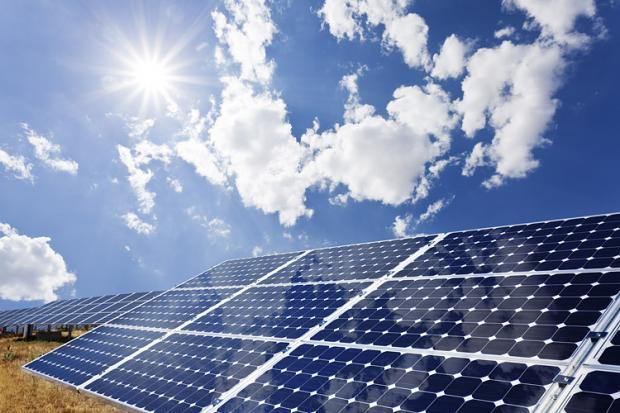
\includegraphics[width=\linewidth]{Titelbild.jpg}
\end{figure}
\vfill

{
\renewcommand\arraystretch{2}
\begin{center}
\begin{tabular}{>{\bf}p{4cm} l}
Hochschule                 &    Hochschule für Technik - FHNW\\
Studiengang                &    Elektro- und Informationstechnik\\
Autor/-en  		           & 	Mischa Knupfer, Andres Minder\\
Betreuer                   &    Prof. Dr. Taoufik Nouri\\
Auftraggeber               &    Prof. Dr. Taoufik Nouri\\
Version                    &    1.0 %Normally not used!
\end{tabular}
\end{center}
}

\clearpage
			
%%---ABSTRACT----------------------------------------------------------------------------
\selectlanguage{english}				%ngerman or english
\thispagestyle{empty}
%\begin{abstract}

\end{abstract}	

%%---TABLE OF CONTENTS-------------------------------------------------------------------
\pagenumbering{Roman}		
\selectlanguage{ngerman}				%ngerman or english
\tableofcontents
\clearpage

%%---TEXT--------------------------------------------------------------------------------
\pagenumbering{arabic}
\section{Ziele P5/P6}

In diesem Abschnitt werden die Muss- und Wunschziele von P5 und P6 tabellarisch dargestellt. Die Ziele von P6 werden erst zu Beginn des P6 näher definiert und nachgetragen.

% Table generated by Excel2LaTeX from sheet 'Tabelle1'
\begin{table}[htbp]
  \centering
  \caption{Ziele P5}
  \small
    \begin{tabular}{r|l|r|l|l}
          & \textbf{Ziel} & \multicolumn{1}{l|}{\textbf{Messbereiche}} & \textbf{Genauigkeiten} & \textbf{Einheiten} \\
    \toprule
    \multicolumn{1}{l}{\textbf{Mussziele P5}} & \multicolumn{1}{r}{} & \multicolumn{1}{r}{} & \multicolumn{1}{r}{} &  \\
    \toprule
    \multicolumn{1}{l|}{Sensoren} & Lufttemperaturmessung & \multicolumn{1}{l|}{[-20;30]} & $\pm$ 0,5 & C \\
          &       & \multicolumn{1}{l|}{[30;100]} & $\pm$ 1   & C \\
\cline{2-5}           & Rel. Luftfeuchtigkeitsmessung & \multicolumn{1}{l|}{[0;50]} & $\pm$ 3   & \% \\
          &       & \multicolumn{1}{l|}{[50;80]} & $\pm$ 2   & \% \\
          &       & \multicolumn{1}{l|}{[80;100]} & $\pm$ 3   & \% \\
\cline{2-5}           & Luftdruckmessung & \multicolumn{1}{l|}{[0;1000]} & $\pm$ 2   & mBar \\
\cline{2-5}          & Windgeschwindigkeitsmessung & \multicolumn{1}{l|}{[0,5;11]} & $\pm$ 1   & m/s \\
    \hline
    \multicolumn{1}{l|}{Datenspeicherung} & Datenabfrage via PuTTY &   $\geq$ 9600    &       &  Bd/s\\
    \hline
    \multicolumn{1}{l|}{RTC} & Implementation &   Echtzeit    & $\pm$ 1   & s/Jahr \\
    \bottomrule
    \multicolumn{1}{l}{\textbf{Wunschziele P5}} & \multicolumn{1}{r}{} & \multicolumn{1}{r}{} & \multicolumn{1}{r}{} &  \\
    \toprule
    \multicolumn{1}{l|}{Sensoren} & Windrichtungsmessung & \multicolumn{1}{l|}{[0;360]} & $\pm$ 20  & ° Winkelmass \\
\cline{2-5}           & Niederschlagsart & \multicolumn{1}{l|}{Regen} & \multicolumn{1}{r|}{100} & \% \\
          &       & \multicolumn{1}{l|}{Hagel} & \multicolumn{1}{r|}{100} & \% \\
          &       & \multicolumn{1}{l|}{Schnee} & \multicolumn{1}{r|}{100} & \% \\
\cline{2-5}           & Niederschlagsmenge &   Wasser    & $\pm$ 100 & mL/m$^2$ \\
\bottomrule
    \end{tabular}%
  \label{tab:ZieleP5}%
\end{table}%

% Table generated by Excel2LaTeX from sheet 'Tabelle1'
\begin{table}[htbp]
  \centering
  \caption{Ziele P6}
  \small
    \begin{tabular}{l|l|r|r|r}
          & \textbf{Ziel} & \multicolumn{1}{l|}{\textbf{Messbereiche}} & \multicolumn{1}{l|}{\textbf{Genauigkeiten}} & \multicolumn{1}{l}{\textbf{Einheiten}} \\
    \toprule
    \multicolumn{1}{l}{\textbf{Mussziele P6}} & \multicolumn{1}{r}{} & \multicolumn{1}{r}{} & \multicolumn{1}{r}{} &  \\
    \toprule
    Speisung & Akkukapazität &       &       &  \\
\cline{2-5}          & Ladeschaltung Akku &       &       &  \\
\cline{2-5}           & Ladeschaltung Photovoltaik &       &       &  \\
    \hline
    Kommunikationsmodul & GPS   &       &       &  \\
\cline{2-5}          & Mobilfunk (SMS) &       &       &  \\
    \bottomrule
    \multicolumn{1}{l}{\textbf{Wunschziele P6}} & \multicolumn{1}{r}{} & \multicolumn{1}{r}{} & \multicolumn{1}{r}{} &  \\
    \toprule
    Kommunikationsmodul & Mobilfunk (Website) &       &       &  \\
    \hline
    Speisung & Netzadapter &       &       &  \\
    \bottomrule
    \end{tabular}%
  \label{tab:ZieleP6}%
\end{table}%


\section{Grundkonzept}
\label{chap:grundkonzept}
\begin{figure}[h]
	\centering
	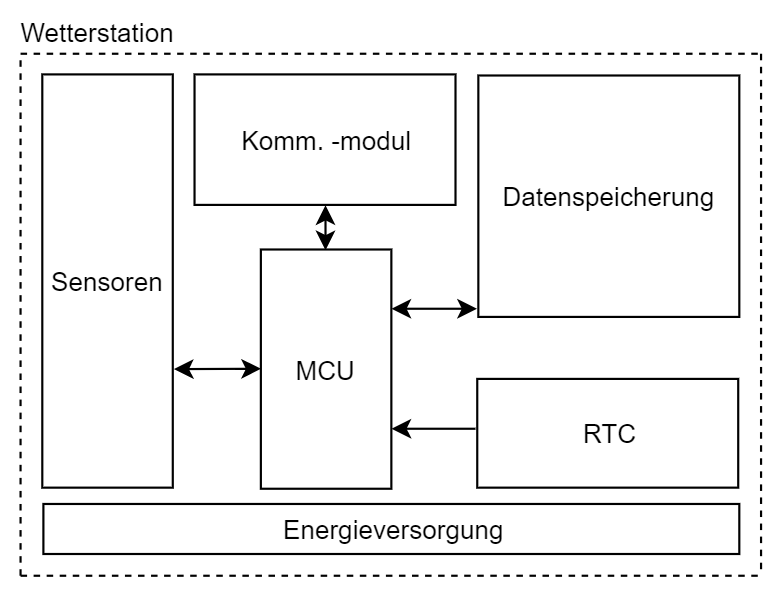
\includegraphics[width=0.9\textwidth]{graphics/Grundkonzept.PNG}
	\caption{Grundkonzept}
	\label{fig:grundkonzept}
\end{figure}

\paragraph{Übersicht:}
Als Zentralrecheneinheit wird eine \textit{Micro-Controller-Unit (MCU)} verwendet. Dieser ist dafür verantwortlich, dass die Daten richtig verarbeitet und an das dementsprechende Modul weitergeleitet werden. Die Messdaten werden in digitaler Form vom Modul \textit{Sensoren} an die \textit{MCU} übertragen. Dieser fügt mit dem \textit{Real-Time-Clock (RTC)} einen Timestamp hinzu, wobei anschließend die Daten in der \textit{Datenspeicherung} nichtflüchtig gespeichert werden. Über das \textit{Kommunikationsmodul} können dann die Daten von Nutznießern abgefragt werden.

\vspace{0.5cm}
\hrule
\vspace{0.25cm}

Das gesamte Grundkonzept ist, wie in der Abbildung \ref{fig:grundkonzept} graphisch Dargestellt, modular aufgebaut. Auf alle einzelnen Module wird folgend spezifischer eingegangen und die Konzeptvariationen vorgestellt. Dafür sind zusätzlich noch Vor- \& Nachteile für die Varianten aufgelistet.\\
\newpage

\subsection{Micro Controller Unit (MCU)}
\paragraph{Variante 1:}
\begin{wrapfigure}{r}{0.5\textwidth}
  \vspace{-10pt}
  \begin{center}
    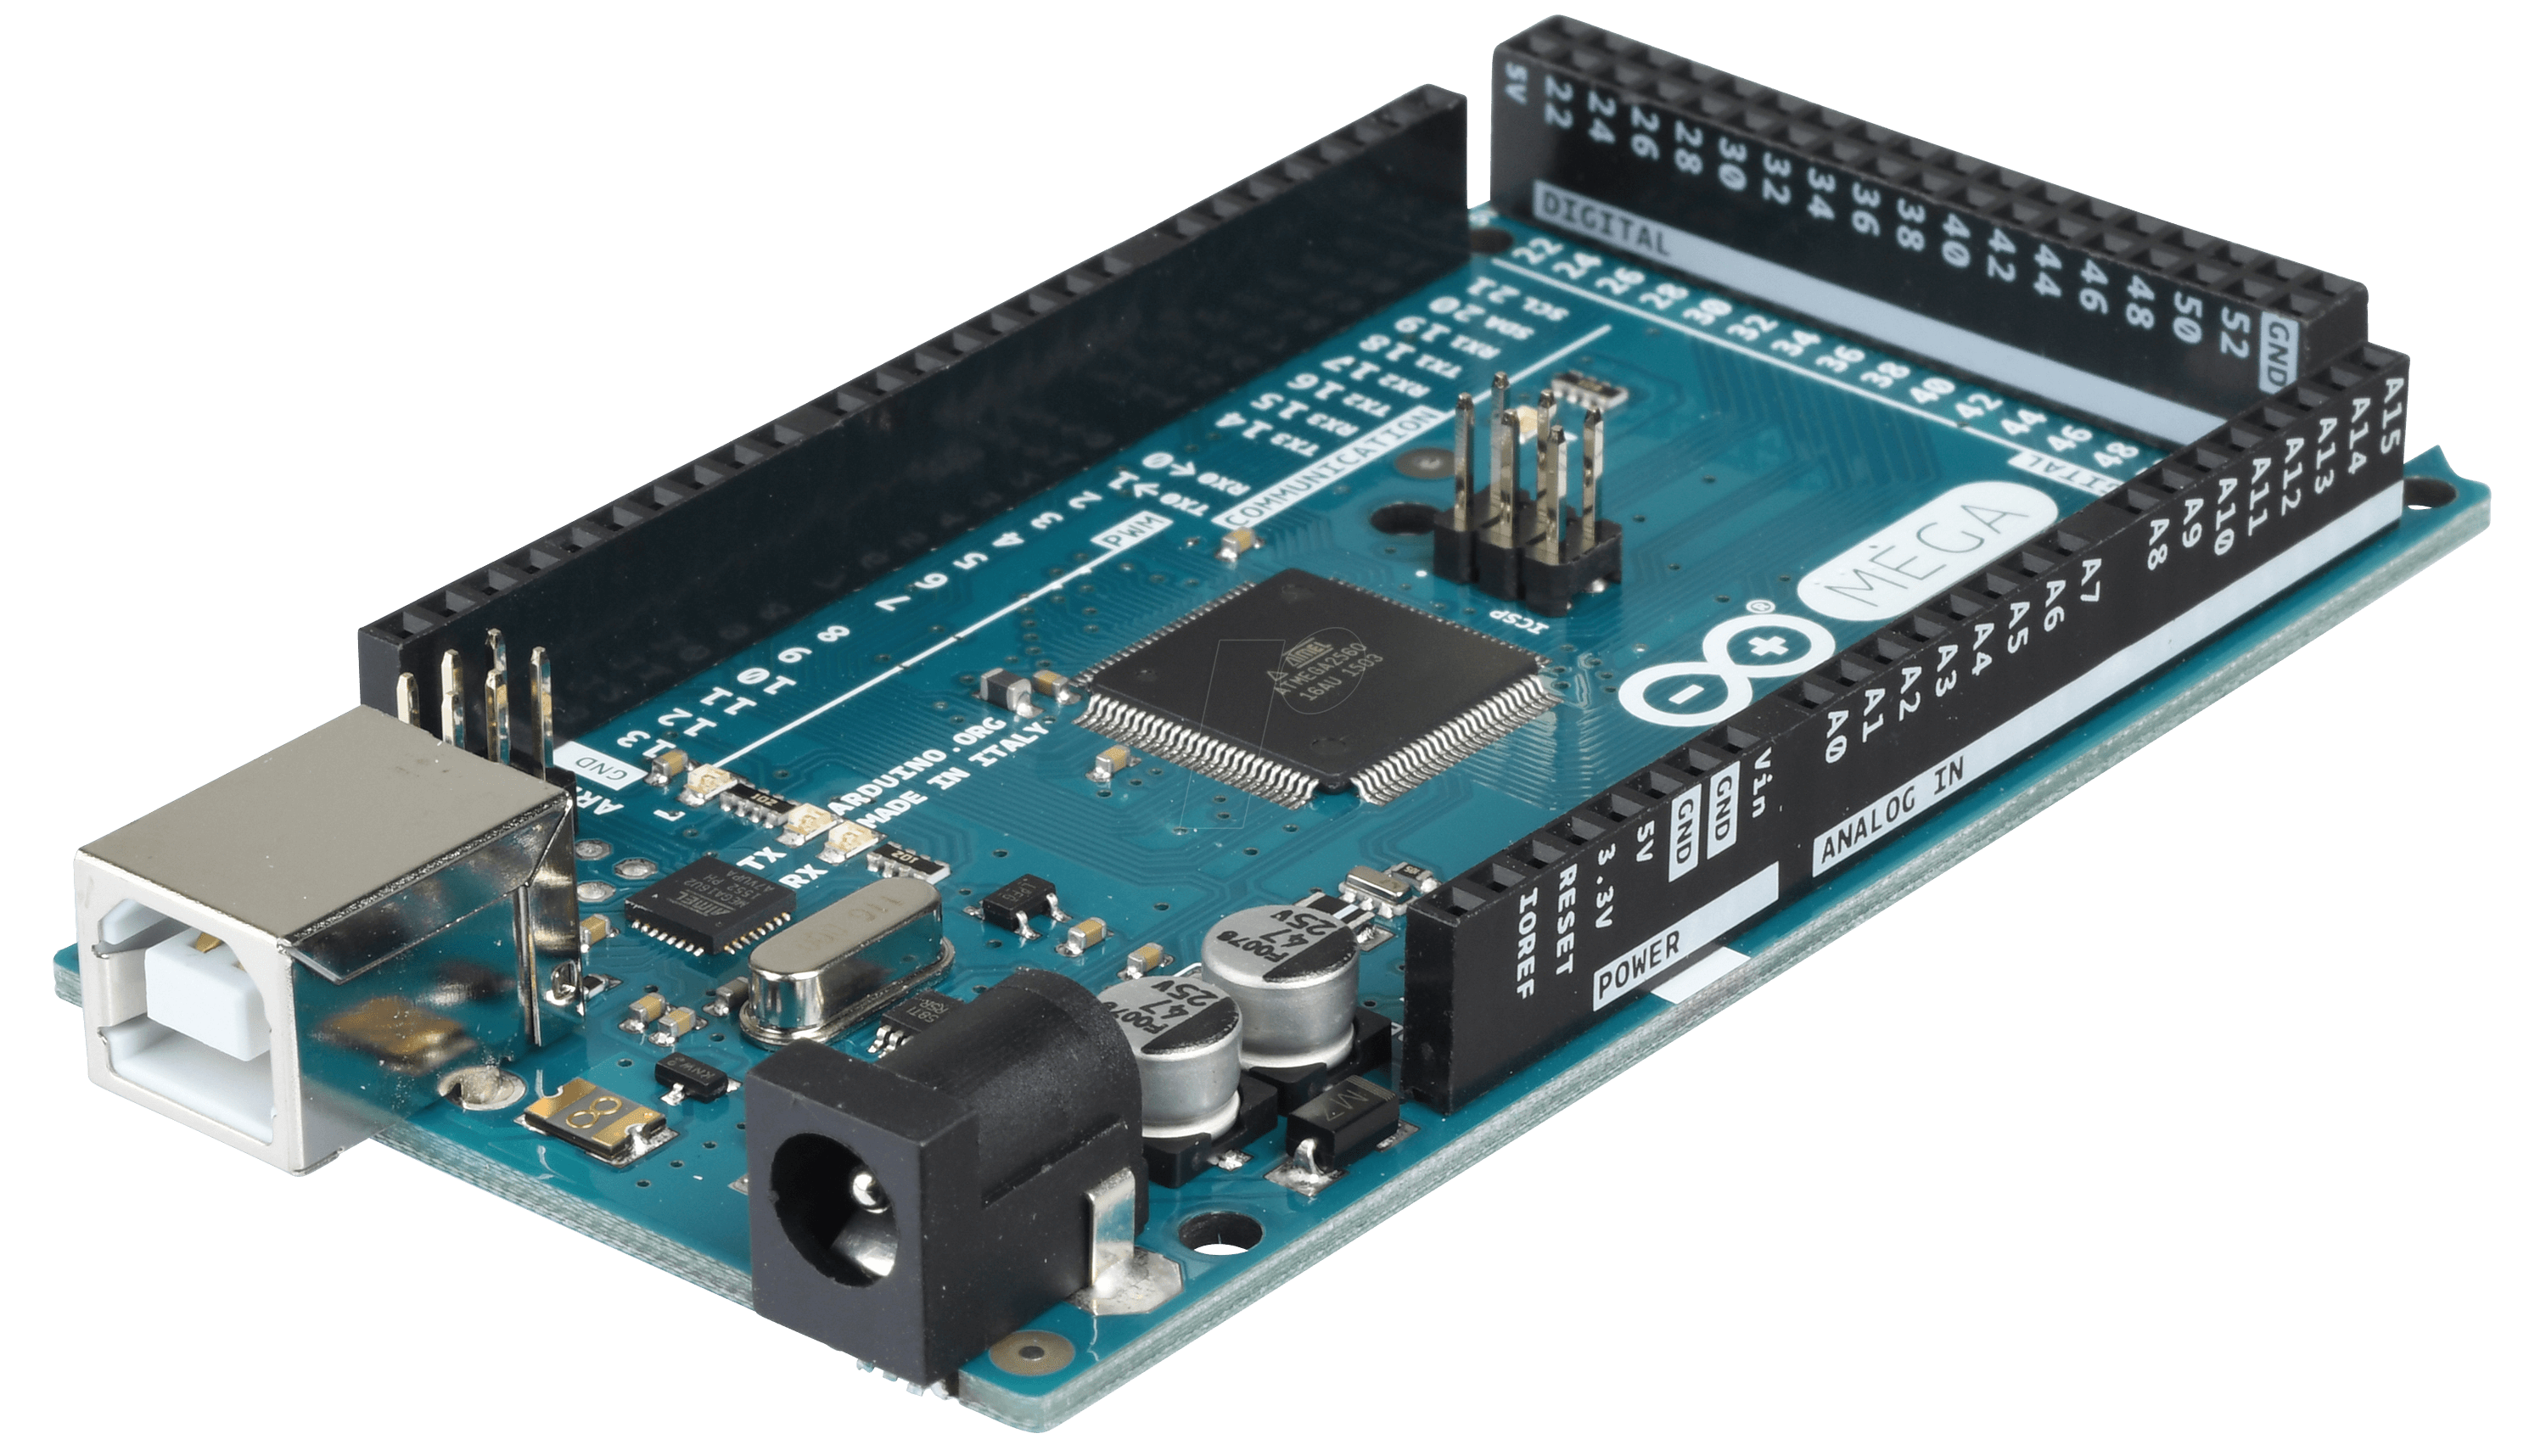
\includegraphics[width=0.38\textwidth]{graphics/arduino_mega.png}
  \end{center}
  \vspace{-10pt}
  \caption{Arduino Mega}
  \vspace{-10pt}
  \label{fig:arduino_mega}
\end{wrapfigure}
Für den \textit{MCU} wird ein ATmega2560 8-bit Microcontroller auf einem Arduino Mega Board implementiert verwendet. Dieser hat 256 KB Flash Memory\footnote{abzüglich 8 KB des Bootloaders} und 8 KB SRAM, was genügend Kapazität für die Implementation der Ablaufsteuerung der Wetterstation bietet. Er oszilliert mit 16 MHz.\\

\paragraph{Variante 2:}

Es wird ein separates Printed Circuit Board (PCB) für die MCU designed. Dafür wird der gleiche Microcontroller wie bei Variante 1 verwendet.\\

\begin{table}[h]
  \centering
  \label{tab:mcu}
  \small
  \caption{Vor- \& Nachteile}
    \begin{tabular}{c|l|l}
          & \textbf{Vorteile} & \textbf{Nachteile} \\
    \toprule
    \multirow{4}[2]{*}{\textbf{Variante 1}} & • in-system Programmierung &  \\
          & \hspace{0.3cm} über USB Typ B möglich &  \\
          & • USB-Schnittstelle für eine &  \\
          &   \hspace{0.3cm} Datenkommunikation mit PC &  \\
    \hline
    \multirow{4}[1]{*}{\textbf{Variante 2}} &       & • zusätzlicher ICSP-Header für \\
          &       & \hspace{0.3cm} eine in-system Programmierung mit \\
          &       & \hspace{0.3cm} einem zusätzlichen Gerät (z.B. AVR Dragon) \\
          &       & • benötigt UART-to-USB Chip \\
    \end{tabular}%
  \label{tab:addlabel}%
\end{table}%

\newpage
\subsection{Sensoren}
\begin{figure}[h]
\centering
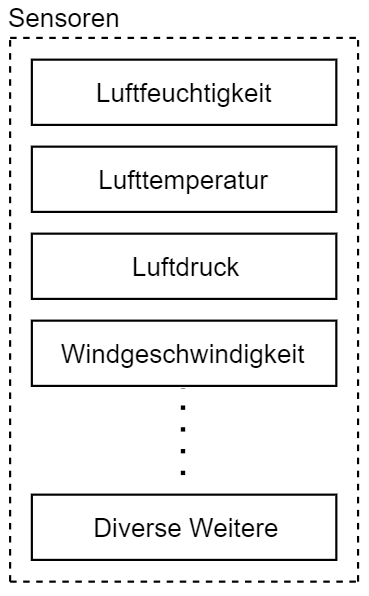
\includegraphics[scale=0.8]{graphics/Sensoren.PNG}
\caption{Sensoren}
\end{figure}

\subsubsection*{Sensoraufbau}
In der Abbildung \ref{fig:sensoraufbau} ist graphisch gezeigt, wie ein einzelner Sensor in etwa aufgebaut ist. 
\begin{figure}[h]
\centering
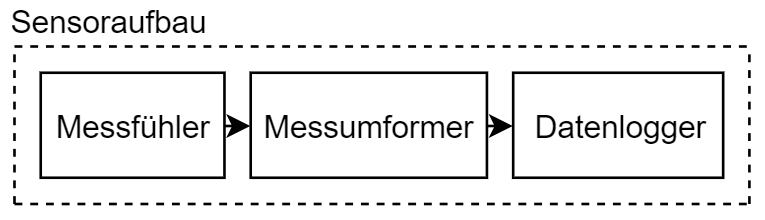
\includegraphics[scale=0.7]{graphics/Sensoraufbau.PNG}
\caption{Sensoraufbau}
\label{fig:sensoraufbau}
\end{figure}

\subsubsection{Temperatursensor}

\subsubsection{Luftfeuchtigkeitssensor}
Die Bestimmung der relativen Luftfeuchtigkeit spielt eine markante Rolle in der Meteorologie. Dieser Wert sagt aus, wie sehr die Luft mit Wasserdampf gesättigt ist und wird mit anderen Faktoren benutzt um zuverlässige lokale Wetterprognosen zu erstellen. Die Normwerte für die Schweiz liegen ungefähr zwischen 58 und 92 Prozent relativer Luftfeuchtigkeit  \cite{MeteoSchweizFeuchte}.\\
Um diesen Wert zu messen, wird ein kapazitiver Absorptionshygrometer verwendet. Diese sind weit verbreitet, besitzen eine passable Genauigkeit (1-3 \% relative Luftfeuchte), sind Robust, wartungsarm und kostengünstig.

\subsubsection{Luftdrucksensor}
Der Luftdruck spielt bei der Erkennung von Hoch- und Tiefdruckgebieten eine wichtige Rolle in der Meteorologie. Diser wird ebenso verwendet um zuverlässige lokale Wetterprognosen zu erstellen. Die Normwerte für die Schweiz liegen ungefähr zwischen 640 und 1000 hPa \cite{MeteoSchweizDruck}.\\
Um diesen Wert zu messen, wird ein Absolutdrucksensor benötigt, welcher den Absolutwert des aufgenommenen Drucks durch Vergleich mit Vakuum als Referenzpunkt ermittelt. Dieses Verfahren ist die einzige Möglichkeit um den atmosphärischen Luftdruck selbst zu messen \cite{WikiDruck}. 

\subsubsection{Windstärke- und Windrichtungssensor}
Die Windstärke (Windgeschwindigkeit) und Windrichtung haben einen Einfluss auf das Wetter und sind aus diesem Grund ebenso von Bedeutung für die Meteorologie. Ausserdem indizieren hohe Windstärke Stürme, weshalb vor allem die Windstärkemessung für Unwetterwarnungen von hoher Bedeutung ist. Die Normwerte für die Schweiz liegen ungefähr zwischen 0.5 und 11 $\frac{m}{s}$ \cite{MeteoSchweizWindnorm}. Wobei bereits Extremwerte mit bis zu 53 $\frac{m}{s}$ im Flachland und bis zu 75 $\frac{m}{s}$ in den Bergen detektiert wurden \cite{MeteoSchweizExtrem}.\\
Um die Windstärke zu messen, wird ein Schalenanemometer verwendet, da diese nicht nach der Windrichtung ausgerichtet werden müssen und nicht so viel Strom benötigen wie auf Ultraschall basierende Sensoren. Die Windrichtung selbst kann mit einer Windfahne detektiert werden, wobei hier die Umsetzung der Richtung in ein digitales Signal weitere Recherche benötigt.

\subsubsection{Niederschlagsensor}

\subsection{Kommunikationsmodul}
\begin{figure}[h]
\centering
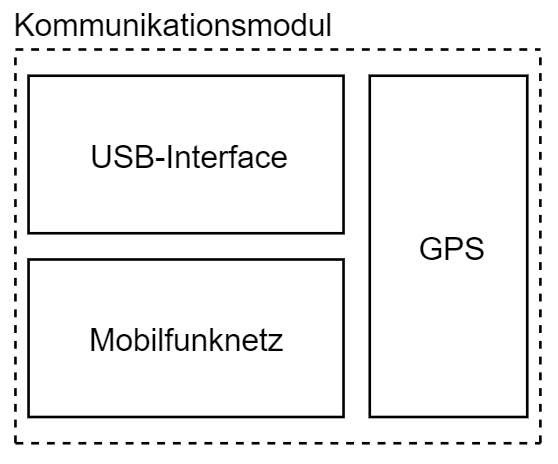
\includegraphics[scale=0.7]{graphics/Kommunikationsmodul.PNG}
\caption{Kommunikationsmodul}
\end{figure}
\newpage
\subsection{Datenspeicherung}
\paragraph{Variante 1:}

Die Datenspeicherung erfolgt auf einer $\mu$SD-Karte. Diese kann in ein Breakoutboard eingeschoben werden.\\

\paragraph{Variante 2:}

Es werden zur Datenspeicherung EEPROM's benutzt.\\

\begin{table}[h]
  \centering
  \label{tab:datenspeicherung}
  \small
  \caption{Vor- \& Nachteile}
    \begin{tabular}{c|l|l}
          & \textbf{Vorteile} & \textbf{Nachteile} \\
    \toprule
    \multirow{4}[2]{*}{\textbf{Variante 1}} & • internes level-shifting & • es wird ein zusätzliches \\
          & • grosser Speicherplatz & \hspace{0.3cm}Breakoutboard verwendet \\
          & • Daten können notfalls auch &  \\
          &   \hspace{0.3cm} direkt von der $\mu$SD-Karte &  \\
          &   \hspace{0.3cm} entnommen werden &  \\
    \hline
    \multirow{2}[1]{*}{\textbf{Variante 2}} &       & • kleiner Speicherplatz \\
          &       & • benötigt level-shifting \\
    \end{tabular}%
  \label{tab:addlabel}%
\end{table}%


\subsection{RTC}

\subsection{Speisung}
\begin{figure}[h]
\centering
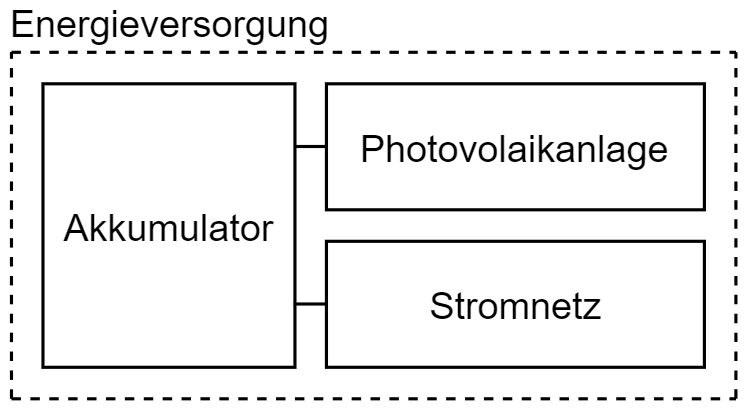
\includegraphics[scale=0.6]{graphics/Energieversorgung.PNG}
\caption{Energieversorgung}
\end{figure}

\section{Verifikationskonzept}

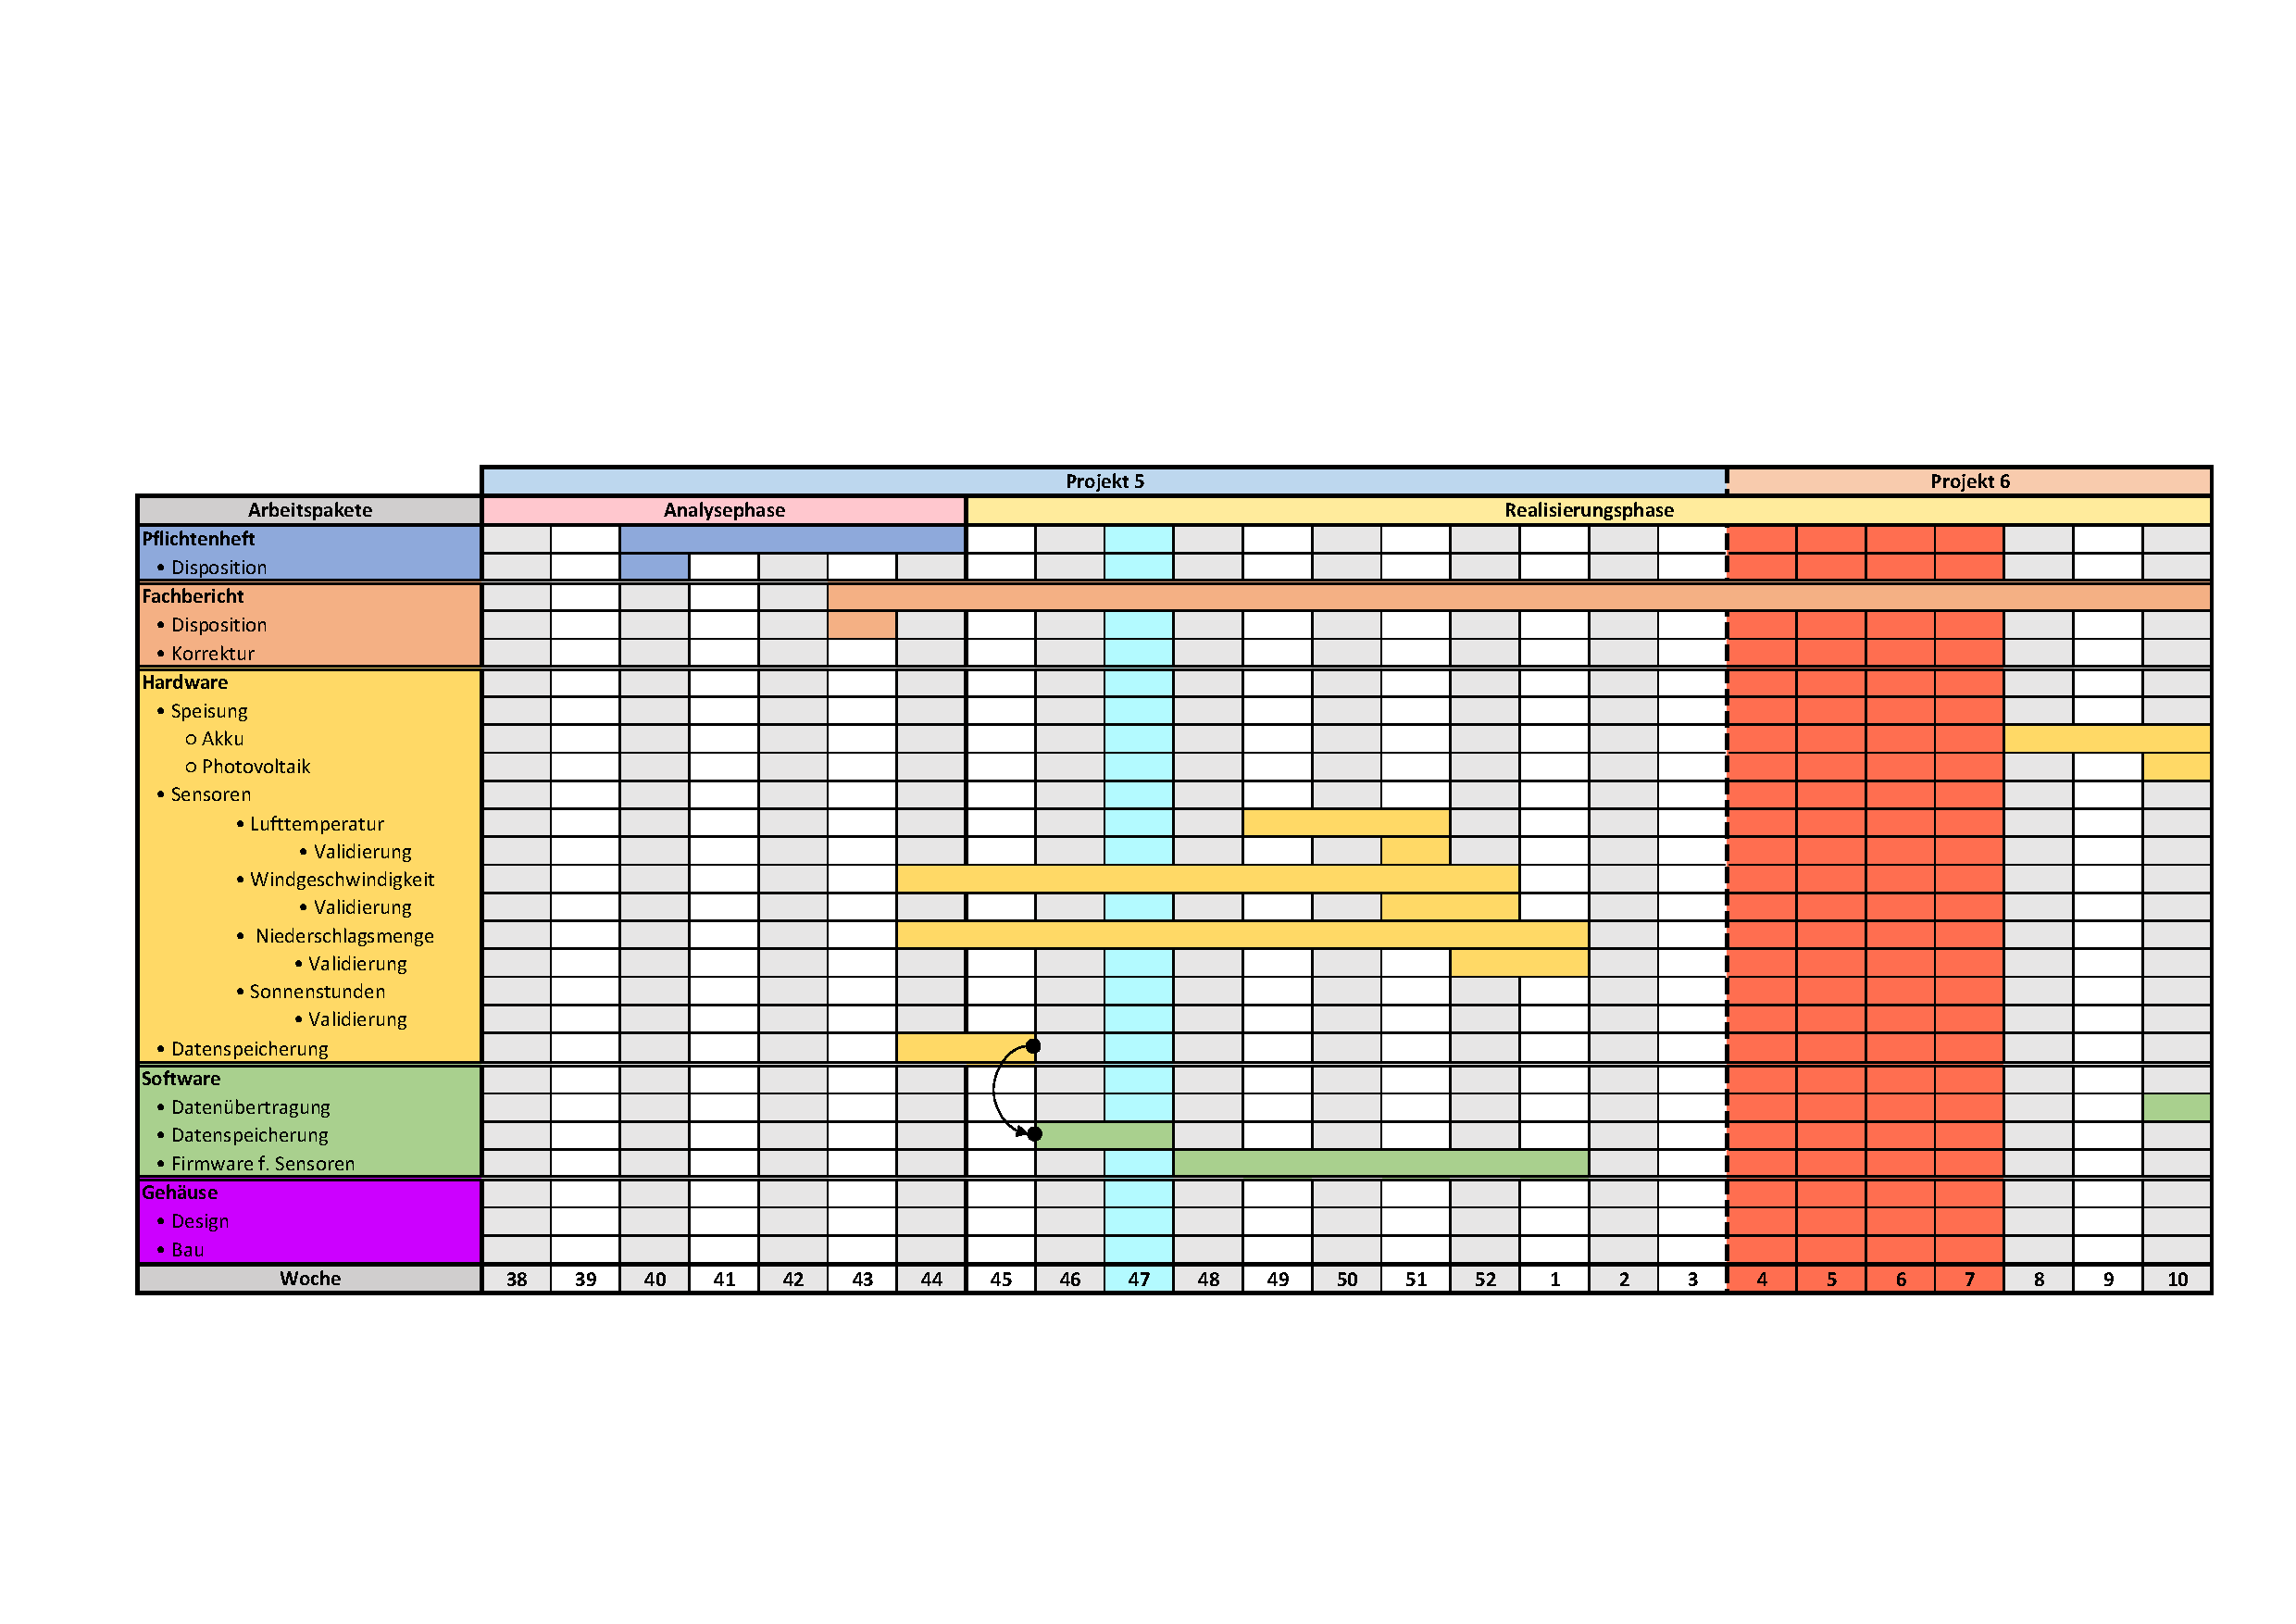
\includepdf[pages={1},nup=1x1,landscape=true,scale=0.85,offset=0 -40,pagecommand={\section{Zeitplan Projektverlauf}\label{tab:zeitplan}\thispagestyle{myheadings}}]{graphics/prov_zeitplanung.pdf} \newpage

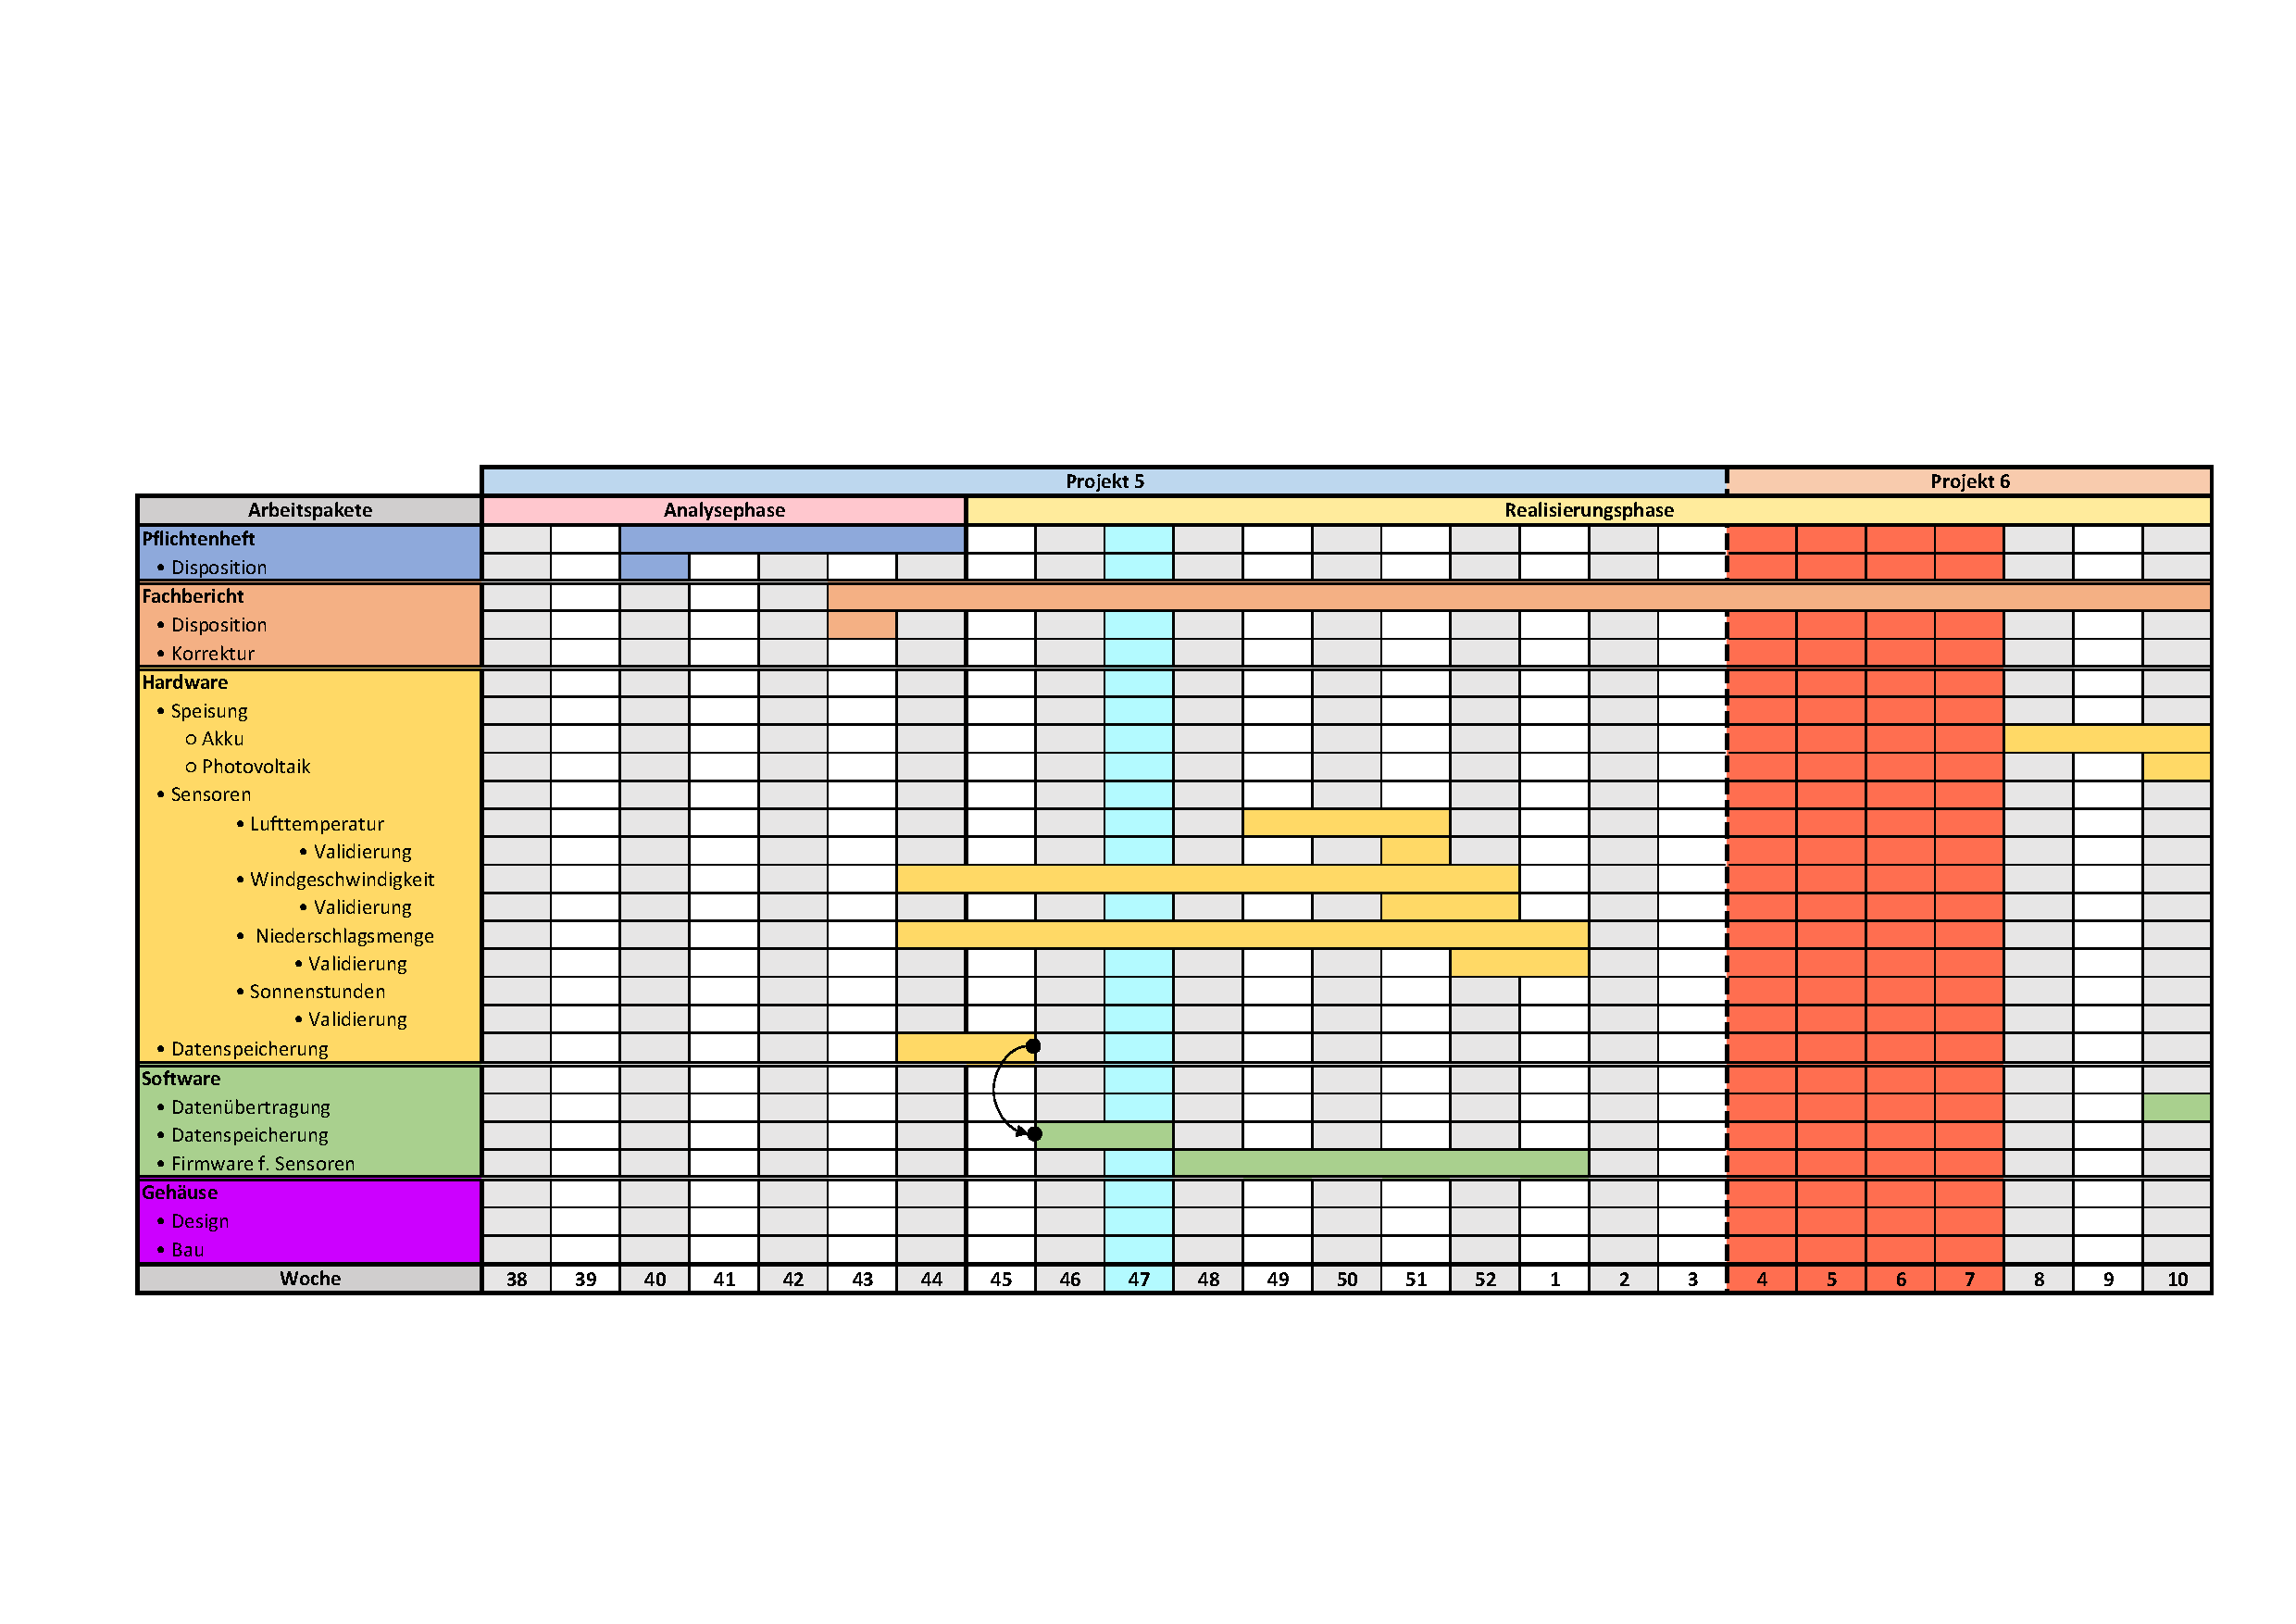
\includepdf[pages={1},nup=1x1,landscape=true,scale=0.85,offset=0 -40,pagecommand={\label{tab:zeitplan}\thispagestyle{myheadings}}]{graphics/prov_zeitplanung.pdf} \newpage

%\section{Budgetplanung}
In einer übersichtlichen Tabelle werden die benötigten Budgets für die unterschiedlichen Gesamtkonzepte aufgeführt. Somit sind die wichtigsten Zahlen zusammengetragen und es bietet sich ein Überblick über die garantiert, anfallenden Kosten.
\section{Risikoanalyse}
In einem Projekt kann es immer wieder zu Problemen führen. In diesem Kapitel wird sich mit diesem Thema auseinandergesetzt und gezeigt, mit welchen Methoden auf die unterschiedlichen Eventualitäten reagiert werden kann.
\section{Kommunikation}
Wichtig innerhalb eines Projektes ist die Kommunikation im Team, sowie zwischen dem Team, Auftraggeber und Berater. Diese werden in diesem Kapitel festgelegt, um auch Missverständnisse zu umgehen.

%%---BIBLIOGRAPHY------------------------------------------------------------------------
\bibliography{literature/bibliography}

%%---APPENDIX----------------------------------------------------------------------------
\begin{appendix}
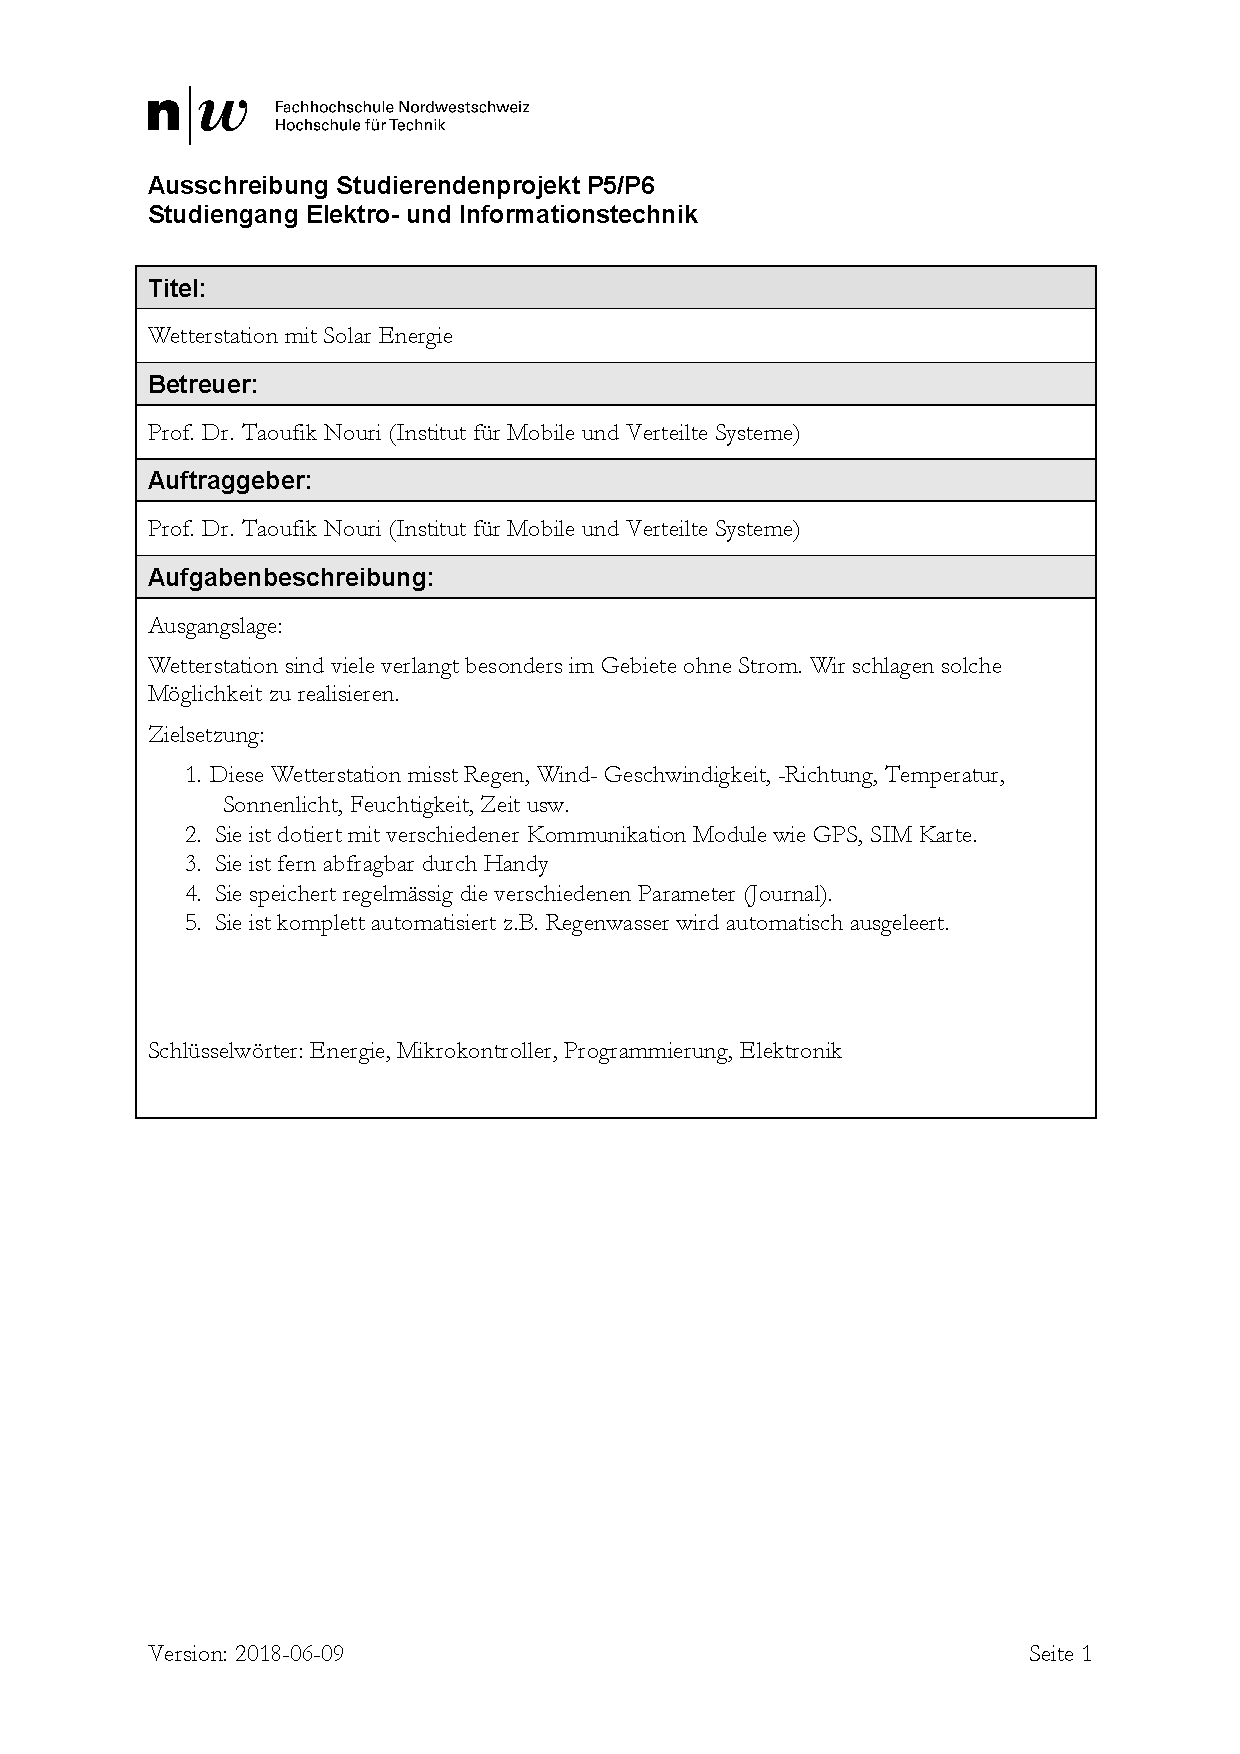
\includepdf[pages={1},nup=1x1,landscape=false,scale=0.85,offset=0 -40,pagecommand={\section{Auftragsbeschreibung}\label{tab:zeitplan}\thispagestyle{myheadings}}]{appendix/Auftragsbeschreibung.pdf} \newpage
\end{appendix}

%%---NOTES for DEBUG---------------------------------------------------------------------
\ifdraft{%Do this only if mode=draft
%%requires \usepackage{todonotes})
\newpage
\listoftodos[\section{Todo-Notes}]
\clearpage
}
{%Do this only if mode=final
}
\end{document}
